\documentclass[parskip=full,11pt,twoside]{scrartcl}
\usepackage[utf8]{inputenc}

\title{VIPER: Viper Interactive Prolog Education Runtime}
\author{Paul Brinkmeier, Luke Brocke, Christian Oder, Aaron Maier, Jannik Koch}

% section numbers in margins:
\renewcommand\sectionlinesformat[4]{\makebox[0pt][r]{#3}#4}

% header & footer
\usepackage{scrlayer-scrpage}
\lofoot{\today}
\refoot{\today}
\pagestyle{scrheadings}

\usepackage{amsmath} % for $\text{}$

\usepackage[sfdefault,light]{roboto}
\usepackage[T1]{fontenc}
\usepackage[german]{babel}
\usepackage[yyyymmdd]{datetime} % must be after babel
\renewcommand{\dateseparator}{-} % ISO8601 date format
\usepackage{hyperref}
\usepackage[nameinlink]{cleveref}
\crefname{figure}{Abb}{Abb}
\usepackage[section]{placeins}
\usepackage{xcolor}
\usepackage{graphicx}
\hypersetup{
	pdftitle={Pflichtenheft},
	bookmarks=true,
}
\usepackage{csquotes}

\newcommand\urlpart[2]{$\underbrace{\text{\texttt{#1}}}_{\text{#2}}$}

\usepackage{pflichtenheft}

\begin{document}
\maketitle

\section{Einleitung}

Einleitende Worte.

\pagebreak
\section{Kriterien}
% Diese Section sollte kurz und knapp "für Manager" sein
% und auf eine Seite passen.

\subsection{Muss}

\criterium{Interpretation eines Prolog-Programms mit begrenztem Umfang}{crt:interpretation}

Das Programm kann eine Teilmenge der Prologsprache interpretieren.

\subsection{Kann}

\criteriumOptional{Export von Visualisierungsbäumen als Bilddatei}{crt:export}

Das Programm kann einen Visualisierungsbaum als Bilddatei im PNG-Format exportieren.

\subsection{Abgrenzung}

\criteriumNot{Voller Sprachsupport}{crt:fullsupport}

Die Software hat kein Verständnis für Prolog-Sprachfeatures außerhalb der vorgestellten Prolog-Teilmenge.

\criteriumNot{Andere Programmiersprachen}{crt:otherlanguages}

Die Entwicklungsumgebung beschränkt sich auf die Prolog-Sprache und bietet keine offiziell Unterstützung für Prolog-Dialekte oder andere Programmiersprachen jeglicher Art.

\criteriumNot{Nutzung in einer Kommandozeile}{crt:cli}

Das Produkt beschränkt sich auf eine graphische Darstellung über GUI-Elemente. Eine Interaktion über die Konsole ist nicht unterstützt.

\criteriumNot{Nicht für professionelle Anwendung}{crt:notforprofessionaluse}

Die Software ist nicht für professionelle Anwendungszwecke ausgelegt. Bei Projekten mit über 2000 Fakten kann es zu Performanceeinbußen kommen.

\pagebreak
%%%%%%%%%%%%%%
\section{Produkteinsatz}

Das Produkt soll als graphisches Prolog-Lerntool betrieben werden.

Die Zielgruppe des Lerntools sind Studierende und Enthusiasten.

Das Produkt soll sich auf eine Teilmenge der Prolog-Sprache beschränken, diese jedoch voll unterstützen.

Das Produkt soll für die Teilmenge der Sprache eine integrierte Entwicklungsumgebung darstellen.

Neben einer Entwicklungsumgebung für die unterstützte Teilmenge von Prolog stehen Visualisierungs-Features zum Verständnis der Sprachumsetzung zur Verfügung.

\section{Produktumgebung}

Das Programm soll als graphische Applikation auf einem Desktop-System betrieben werden.

Es stehen mindestens 2 AMD64/x86 Kerne mit insgesamt 2GB shared RAM zur Verfügung.

Unterstützte Betriebssysteme sind Windows ab Version 7 und aufwärts, Mac OSX 10.9 aufwärts sowie Ubuntu Linux 16.04.

Eine Maus sowie eine Tastatur sind als Eingabegeräte angeschlossen und funktionsfähig.

Eine Installation des Java Runtime Environments Version 8 aufwärts ist auf dem System vorhanden.

%%%%%%%%%%%
\section{Funktionale Anforderungen}

\functionality{Importieren einer oder mehrerer Prolog Quellcode Datei(en)}{fnc:open}
\fulfills{crt:open}

Zu Verwendung des Prolog Interpreters muss eine Datei mit Fakten geladen oder im Editor selbst erstellt werden. Werden mehrere Dateien geöffnet, so werden diese automatisch in verschiedenen Tabs organisiert.

\functionality{Automatische Vervollständigung von Eingaben im Editor}{fnc:autocompletion}
\fulfills{crt:autocompletion}

Das Schreiben von Programmen wird durch die automatische Vervollständigung vereinfacht. Vorgeschlagen werden z.B. bisher definierte Fakten und bekannte Namen.

\functionality{Konfigurieren der Formatierung des Quellcodes.}{fnc:formatter}
\fulfills{crt:formatter}

In einem Einstellungs-Dialog kann die Formatierung des Quellcodes den Präferenzen des Benutzern angepasst werden. Dazu gehören beispielsweise die Einrückungstiefe von neuen Zeilen oder die Verwendung von Tabs statt Leerzeichen zur Einrückung.

\functionality{Verändern und Speichern von Änderungen an einer Prolog Datei.}{fnc:save}
\fulfills{crt:save}

Die Software kann Änderungen an den geöffneten Dateien zurück auf die Festplatte schreiben, damit die entstehende oder überschriebene Datei in anderen Weisen weiterverwendet werden kann.

\functionality{Interpretieren einer im Editor geöffneten Prolog Datei durch einen eigenen Interpreter}{fnc:interpreter}
\fulfills{crt:interpreter}

Die aktuell geöffnete Datei kann mittels einem eigenen Interpreter ausgeführt werden. Der Parser erkennt dabei syntaktische Fehler und prangert diese an.

\functionality{Eingabe von Prolog-Abfragen in der Konsole mit entsprechender Antwort des Interpreters}{fnc:ask}
\fulfills{crt:ask}

Bei erfolgreicher Interpretation einer Datei ohne Fehler stellt die Konsole die Möglichkeit zur Abfrage von beispielsweise Fakten nach Prolog-Syntax bereit.

\functionality{Visualisieren der letzten Prolog-Abfrage mittels eines Graphen}{fnc:slider}
\fulfills{crt:slider}

Die letzte Abfrage, die durch die Konsole eingegeben wurde, wird in einem seperaten Fenster grafisch aufbereitet, um beim Verständnis von Prolog und speziell der Interpretation von Programmen zu unterstützen.

\functionality{Auswahl des anzuzeigenden Interpretations-Schritts für den Graphen.}{fnc:slider}
\fulfills{crt:slider}

Der gewünschte Interpretations-Schritt kann durch eine Leiste über alle möglichen Schritte ausgewählt werden, wodurch sich der angezeigte Graph aktualisiert.

\functionality{Debuggen des Prolog Programmes durch Limitierung der interpretierten Fakten.}{fnc:debugger}
\fulfills{crt:debugger}

\functionality{Vergrößern, Verkleinern und Bewegen des visualisierten Graphen durch Bewegungen mit der Maus}{fnc:zoom}
\fulfills{crt:zoom}

Über die Verwendung des Mausrads lässt sich der angezeigte Ausschnitt des Graphen vergrößern und verkleinern. Durch drücken und halten der linken Maustaste lässt sich der angezeigte Ausschnitt auch bewegen.

\functionality{Exportieren des im Editor geöffneten Prolog Quellcodes als LaTeX Code}{fnc:latexexport}
\fulfills{crt:latexexport}

Der aktuell geöffnete Prolog Code lässt sich durch ein Dialogfenster als \LaTeX\ Code exportieren.

\functionality{Exportieren der angezeigten Visualisierung in einem beliebigen Schritt als Grafik und LaTeX Code}{fnc:imageexport}
\fulfills{crt:imageexport}

Der aktuell angezeigte Graph lässt sich durch ein Dialogfenster als Bild exportieren, wahlweise zzgl. mit \LaTeX\ Code für die direkte Einbindung.

\functionality{Syntax-Highlighting im Editor mittels verschiedener Farben und Schrifteffekte}{fnc:syntaxhighlighting}
\fulfills{crt:syntaxhighlighting}

\functionality{Einstellen von Farbe der grafischen Oberfläche}{fnc:themes}
\fulfills{crt:themes}

\functionality{Setzen von Break-Points für den Debugger}{fnc:breakpoints}
\fulfills{crt:breakpoints}

%%%%%%%%%%%
\section{Nicht-Funktionale Anforderungen}

\nonFunctionality{Die VIPER Software startet auf einem modernen System innerhalb von 3 Sekunden und ist voll einsatzbereit.}{nfc:startup}

\nonFunctionality{Ein importiertes oder geschriebnes Prolog Programm ohne Verwendung von Rekursion und im Umfang von maximal 100 Zeilen Code ist innerhalb von maximal 3 Sekunden interpretiert und innerhalb von weiteren 5 Sekunden visualisiert.}{nfc:timelimit}

\nonFunctionality{Das Design wirkt modern und ansprechend.}{nfc:design}

\nonFunctionality{Durch eine englische Übersetzung und die Verwendung von aussagekräftigen Symbolen können auch internationale Studierende ohne ausreichende Deutschkentnisse die Software bedienen.}{nfc:translation}

\nonFunctionality{Die Software lässt sich ohne die manuelle Installation weiterer Software durch das Ausführen einer .jar Datei starten.}{nfc:installation}

\nonFunctionality{Die Software ist ohne Abhängigkeiten kleiner als 50 MiB, mit Abhängigkeiten kleiner als 200 MiB.}{nfc:filesize}

\nonFunctionality{Das Laden einer Prolog Datei mit einer Größe von unter 1 MiB geschieht in unter 5 Sekunden.}{nfc:loadfile}

\nonFunctionality{Das Hauptfenster des Programms lässt sich mit der Maus dynamisch skalieren.}{nfc:resizeable}

\nonFunctionality{Fehlerhafte Prolog-Programme sollen nie zu einem Absturz des Programms führen.}{nfc:crashresistance}

\nonFunctionality{Der Prolog Interpreter lässt sich in seiner Funktionalität einfach erweitern, um weitere Sprachfeatures zu unterstützen.}{nfc:extendable}

\pagebreak
\section{Tests}

\test{Formatierung von Quellcode}{tst:formatter}
\tests{fnc:formatter}

\teststep{Der Nutzer hat einen Quelltext im Editor eingegeben oder aus einer Datei geladen.}
{Der Nutzer betätigt den Formatieren-Button in der oberen Leiste des Hauptfensters.}
{Der Quelltext wird automatisch nach fest definierten Regeln formatiert.}

%%%%%%%%%%%%%%%%%%%%%%%%%%%%%%%%%%%%%%%%%%%%%%%%%%%%%%%%%%%%%%%%%%%%%%%

\test{Öffnen einer Prolog-Textdatei}{tst:open}
\tests{fnc:open}

\teststep{Das Programm wird ausgeführt und ist fokussiert. Es ist kein Programm im Editor geöffnet.}
{Der Nutzer wählt über das Datei-Kontextmenü die Öffnen-Funktion aus.}
{Ein Datei-Auswahldialog öffnet sich.}

\teststep{Der Nutzer hat eine Datei über das Auswahlfenster ausgewählt.}
{Der Nutzer betätigt den Öffnen-Button.}
{Die Datei wird im Editor-Fenster geöffnet.}

%%%%%%%%%%%%%%%%%%%%%%%%%%%%%%%%%%%%%%%%%%%%%%%%%%%%%%%%%%%%%%%%%%%%%%%

\test{Öffnen einer Prolog-Textdatei während im Editor bereits ein Programm eingegeben wurde mit Speichern des geschriebenen Programmes}{tst:openanother}
\tests{fnc:open}

\teststep{Das Programm wird ausgeführt und ist fokussiert. Im Editor wurde ein Programm händisch eingegeben.}
{Der Nutzer wählt über das Datei-Kontextmenü die Öffnen-Funktion aus.}
{Ein Datei-Auswahldialog öffnet sich.}

\teststep{Der Nutzer hat eine Datei über das Auswahlfenster ausgewählt.}
{Der Nutzer betätigt den Öffnen-Button.}
{Ein Dialogfenster fragt den Nutzer, ob das im Editor eingegebene Programm gespeichert oder verworfen werden soll.}

\teststep{Der Nutzer hat die Wahl das im Editor geschriebene Programm zu speichern oder zu verwerfen.}
{Der Nutzer betätigt den Speichern-Knopf.}
{Ein Datei-Speichern-Dialog öffnet sich.}

\teststep{Ein Datei-Speichern-Dialog ist geöffnet.}
{Der Nutzer wählt einen Speicherort und wählt einen Dateinamen. Anschließend betätigt es den Speichern-Knopf.}
{Das im Editor geöffnete Programm wird in die gewählte Datei gespeichert. Die zu öffnende Datei wird in den Editor geladen und überschreibt den bisherigen Inhalt.}

%%%%%%%%%%%%%%%%%%%%%%%%%%%%%%%%%%%%%%%%%%%%%%%%%%%%%%%%%%%%%%%%%%%%%%%

\test{Öffnen einer Prolog-Textdatei während im Editor bereits ein Programm eingegeben wurde mit Verwurf des geschriebenen Programmes.}{tst:openanother2}
\tests{fnc:open}

\teststep{Das Programm wird ausgeführt und ist fokussiert. Im Editor wurde ein Programm händisch eingegeben.}
{Der Nutzer wählt über das Datei-Kontextmenü die Öffnen-Funktion aus.}
{Ein Datei-Auswahldialog öffnet sich.}

\teststep{Der Nutzer hat eine Datei über das Auswahlfenster ausgewählt.}
{Der Nutzer betätigt den Öffnen-Button.}
{Ein Dialogfenster fragt den Nutzer, ob das im Editor eingegebene Programm gespeichert oder verworfen werden soll.}

\teststep{Der Nutzer hat die Wahl das im Editor geschriebene Programm zu speichern oder zu verwerfen.}
{Der Nutzer betätigt den Verwerfen-Knopf.}
{Das im Editor geöffnete Programm wird verworfen. Die zu öffnende Datei wird in den Editor geladen und überschreibt den bisherigen Inhalt.}

%%%%%%%%%%%%%%%%%%%%%%%%%%%%%%%%%%%%%%%%%%%%%%%%%%%%%%%%%%%%%%%%%%%%%%%

\test{Speichern eines im Editor geschrieben Programmes}{tst:save}
\tests{fnc:save}

\teststep{Das Programm wird ausgeführt und ist fokussiert. Ein Programm ist im Editor geöffnet.}
{Der Nutzer wählt über das Datei-Kontextmenü die Speichern-Funktion aus.}
{Ein Datei-Speichern-Dialog öffnet sich.}

\teststep{Ein Datei-Speichern-Dialog ist geöffnet.}
{Der Nutzer wählt einen Speicherort und Dateinamen aus. Anschließend bestätigt er den Speichern-Button.}
{Der Inhalt des Editors wird an den gewählten Ort geschrieben}

%%%%%%%%%%%%%%%%%%%%%%%%%%%%%%%%%%%%%%%%%%%%%%%%%%%%%%%%%%%%%%%%%%%%%%%

\test{Interpretierung vom Familie-Simpson-Beispielprogramm}{tst:simpsons}
\tests{fnc:interpreter}

\teststep{Das Familie Simpson Beispielprogramm ist im Editorfenster eingegeben oder aus einer Datei geladen worden.}
{Der Nutzer klickt auf die Parse-Schaltfläche des Hauptfensters.}
{Das Programm wird erfolgreich geparst, es kommt zu keinen Fehlern. Die Konsole erwartet eine Eingabe.}

\teststep{Das Programm wurde geparst und die Konsole erwartet eine Eingabe.}
{Der Nutzer gibt die Abfrage \texttt{father(X, bart).} in der Konsole ein.}
{Das Programm wird interpretiert und zeigt das Ergebnis \texttt{X = homer .} an.}

%%%%%%%%%%%%%%%%%%%%%%%%%%%%%%%%%%%%%%%%%%%%%%%%%%%%%%%%%%%%%%%%%%%%%%%

\test{Interaktive Nutzung des Interpreters}{tst:ask}
\tests{fnc:ask}

\teststep{Der Nutzer hat ein fehlerloses Prolog-Programm im Editor eingetragen.}
{Der Nutzer betätigt den Run-Button des Hauptfensters.}
{Die Ausgabe des Prolog-Programmes wird im Interpreter-Fenster angezeigt.}

\teststep{Ein Prolog-Programm wurde im Interpreter ausgeführt. Der Interpreter hat die aktuellen Fakten geladen und eine offene Interpreter-Shell steht bereit.}
{Der Nutzer gibt eine weitere Anfrage ein und bestätigt die Eingabe.}
{Der Interpreter gibt die Antwort auf die Anfrage mit Bezug auf die Fakten des bisherigen Prolog-Programmes zurück.}

%%%%%%%%%%%%%%%%%%%%%%%%%%%%%%%%%%%%%%%%%%%%%%%%%%%%%%%%%%%%%%%%%%%%%%%

\test{Visualisierung eines Programms}{tst:slider}
\tests{fnc:slider}

\teststep{Der Nutzer hat ein gültiges Prolog-Programm in den Editor eingetragen.}
{Der Nutzer betätigt die Visualisierungs-Schaltfläche.}
{Ein Fenster mit einem interaktiven Visualisierungsbaum öffnet sich.}

\teststep{Der Nutzer hat einen interaktiven Visualisierungsbaum für das Programm geöffnet.}
{Der Nutzer betätigt die Schließen-Schaltfläche des neuen Fensters.}
{Das neue Fenster schließt sich. Das Hauptfenster bleibt geöffnet und unverändert.}


%%%%%%%%%%%%%%%%%%%%%%%%%%%%%%%%%%%%%%%%%%%%%%%%%%%%%%%%%%%%%%%%%%%%%%%

\test{Bewegung innerhalb eines Visualisierungsbaumes}{tst:zoom}
\tests{fnc:zoom}

\teststep{Der Nutzer hat ein Programm im Editor eingetragen und das Visualisierungsfenster zu diesem Programm geöffnet.}
{Der Nutzer bewegt das Mausrad zu sich bzw. nach hinten.}
{Die Visualisierungsanzeige zoomt heraus.}

\teststep{Der Nutzer hat ein Programm im Editor eingetragen und das Visualisierungsfenster zu diesem Programm geöffnet.}
{Der Nutzer bewegt das Mausrad von sich weg bzw. nach vorne.}
{Die Visualisierungsanzeige zoomt herein.}

\teststep{Der Nutzer hat ein Programm im Editor eingetragen und das Visualisierungsfenster zu diesem Programm geöffnet.}
{Der Nutzer hält die linke Maustaste gedrückt und bewegt die Maus..}
{Die Visualisierungsanzeige bewegt sich passend zu der Mausbewegung.}


%%%%%%%%%%%%%%%%%%%%%%%%%%%%%%%%%%%%%%%%%%%%%%%%%%%%%%%%%%%%%%%%%%%%%%%

\test{Export als LaTeX für Foliensätze}{tst:latexexport}
\tests{fnc:latexexport}

\teststep{Ein Programm ist im Editor geöffnet und eine Anfrage als Graph visualisiert.}
{Der Nutzer wählt über das Datei-Kontextmenü die LaTeX-Exportieren-Funktion aus.}
{Ein Auswahl-Dialog öffnet sich}

\teststep{Ein Dialog mit den Auswahlmöglichkeiten \enquote{SVG} und \enquote{PNG} ist geöffnet}
{Der Nutzer wählt eine der beiden Optionen aus. Anschließend betätigt er den Speichern-Knopf.}
{Ein Datei-Speichern-Dialog öffnet sich.}

\teststep{Ein Datei-Speichern-Dialog mit ist geöffnet.}
{Der Nutzer wählt eine Dateipfad aus und gibt einen Dateinamen ein. Anschließend betätigt den Speichern-Button.}
{Die visualisierte Graph wird im ausgewählten Format an den gewählten Ort gespeichert. Die passende \texttt{.svg} bzw. \texttt{.png} Dateieendung wird wenn nötig ergänzt.}

%%%%%%%%%%%%%%%%%%%%%%%%%%%%%%%%%%%%%%%%%%%%%%%%%%%%%%%%%%%%%%%%%%%%%%%

\test{Syntaktische Hervorhebung von Prolog-Stichworten}{tst:syntaxhighlighting}
\tests{fnc:syntaxhighlighting}

\teststep{Der Nutzer hat ein leeres Editor-Fenster vor sich.}
{Der Nutzer gibt ein gültiges Prolog Programm im Editor ein.}
{Der Code wird farblich passend hervorgehoben. Identifier und Variablen werden dabei unterschiedlich zu Zahlen eingefärbt. Ebenfalls unterscheiden sich die Farben von umschließenden Klammern. Die Operatoren \texttt{=}, \texttt{:-}, \texttt{is} und \texttt{!} sind farblich von allem anderen unterscheidbar.}

%%%%%%%%%%%%%%%%%%%%%%%%%%%%%%%%%%%%%%%%%%%%%%%%%%%%%%%%%%%%%%%%%%%%%%%

\test{Inkorrektes Prolog-Programm}{tst:syntaxcheck}
\tests{fnc:syntaxcheck}

\teststep{Der Nutzer hat ein inkorrektes Prolog-Programm in den Editor eingetragen.}
{Der Nutzer betätigt die Parse-Schaltfläche, um das Programm zu parsen.}
{Die Ausführung wird abgebrochen und eine verständliche Fehlermeldung wird in der Konsole angezeigt.}

% TODO: Systemtests (komplette Abläufe)

%%%%%%%%%%%%%
\pagebreak
\appendix

\section{Seitenentwürfe}

\begin{figure}[hb]
\fbox{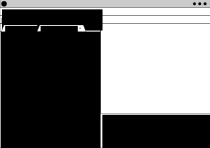
\includegraphics[width=\textwidth]{image/main_view.png}}
\caption{\label{fig:editor}
Hauptfenster
}
\end{figure}

\section{Glossar}

\textbf{Nutzer}:
Eine Person, welche den Dienst nutzt.

\end{document}
